%%%%%%%%%%%%%%%%%%%% author.tex %%%%%%%%%%%%%%%%%%%%%%%%%%%%%%%%%%%
%
% sample root file for your "contribution" to a contributed volume
%
% Use this file as a template for your own input.
%
%%%%%%%%%%%%%%%% Springer %%%%%%%%%%%%%%%%%%%%%%%%%%%%%%%%%%


% RECOMMENDED %%%%%%%%%%%%%%%%%%%%%%%%%%%%%%%%%%%%%%%%%%%%%%%%%%%
\documentclass[graybox]{svmult}

% choose options for [] as required from the list
% in the Reference Guide

\usepackage{type1cm}        % activate if the above 3 fonts are
                            % not available on your system
%
\usepackage{makeidx}         % allows index generation
\usepackage{graphicx}        % standard LaTeX graphics tool
                             % when including figure files
\usepackage{multicol}        % used for the two-column index
\usepackage[bottom]{footmisc}% places footnotes at page bottom


\usepackage{newtxtext}       % 
\usepackage{newtxmath}       % selects Times Roman as basic font

% see the list of further useful packages
% in the Reference Guide

\makeindex             % used for the subject index
                       % please use the style svind.ist with
                       % your makeindex program
\linespread{1.5}

\usepackage[comma,numbers,sort&compress]{natbib}

%\usepackage[style=chem-acs, backend=bibtex]{biblatex}
%\setkeys{chem-acs}{articletitle = true}
%\addbibresource{thesis_ref2.bib}

%%%%%%%%%%%%%%%%%%%%%%%%%%%%%%%%%%%%%%%%%%%%%%%%%%%%%%%%%%%%%%%%%%%%%%%%%%%%%%%%%%%%%%%%%

\begin{document}

\title*{Molecular simulations of biomolecules: some useful guidelines}
\titlerunning{Molecular simulations of biomolecules}
\author{Irene Marzuoli and Franca Fraternali}
% Use \authorrunning{Short Title} for an abbreviated version of
% your contribution title if the original one is too long
\institute{Irene Marzuoli \at Randall Center for Cell and Molecular Biophysics, King's College London, UK \email{irene.marzuoli@kcl.ac.uk}
\and Franca Fraternali \at Randall Center for Cell and Molecular Biophysics, King's College London, UK \email{franca.fraternali@kcl.ac.uk}}
%
% Use the package "url.sty" to avoid
% problems with special characters
% used in your e-mail or web address
%
\maketitle

\abstract{In studying biological processes and focusing on the molecular mechanisms at the basis of these, Molecular Dynamics simulations(MD) have demonstrated to be a very useful tool for the past 50 years. This suite of computational methods calculates the time dependent evolution  of a molecular system using physics-based first principles. In this chapter, we give a brief introduction to the theory and practical use of Molecular Dynamics simulations, highlighting the different models and algorithms that have been developed to tackle specific problems, with a special focus on classical force fields. Some examples of how simulations have been used in the past will help the reader in discerning their power, limitations and significance.}


\section{Introduction}

Molecular Dynamics simulations have been rightly defined as the `Computational Microscope' \cite{Lee2009,Dror2012} as they offer otherwise inaccessible insights into the molecular details underlying conformational changes of proteins and nucleic acids. Computational methods and tools based on MD are routinely applied in structural biology to quantitatively characterise the dynamics and thermodynamics of proteins and their complexes. The increasing computational power available, and the flexibility of the algorithms for implementation on different platforms, have made possible to access molecular dynamical properties inaccessible to experiments. These techniques and the associated force fields are also commonly used in the process of structure determination from NMR data and theoretical structure prediction \cite{Vogel2017,Heo2018}.
%
Modelling and simulating a biological system consists in describing its components and their mutual interactions, and implementing the laws of physics to reproduce its natural evolution. A quantum mechanic description of the system would be more accurate but expensive to achieve for large systems. To facilitate the task, several simplified models have been devised, each most suitable to investigate particular cases.
%
In particular, a large class of models focuses on a classical mechanics description of the dynamics: for increasing sizes of the systems and longer time spans described, the classical approximations will be more than accurate, and also the only possible representation computationally affordable.

Understanding the methodology of classical Molecular Dynamics (MD) provides the interpretative key with which simulations must be designed, run and interpreted in each specific case. We offer here some general background and directions on which are the used algorithms and their applicability in some selected scenarios that we consider representative and challenging.


\section{Materials}

\subsection{Extracting the Dynamics of a Molecular System: the Time Evolution Algorithm}
In a classical MD framework, Newton's second law of motion rules the dynamics, stating that the acceleration $\textbf{a}$ that a particle is subject to at time $t$, depends on the total force $\textbf{F}$ acting on the particle itself and on its mass $m$ (bold denotes vectorial quantities):
\begin{equation} \label{eq:newton}
\textbf{F}(t) =  m \cdot \textbf{a}(t) \, .
\end{equation}
As the acceleration $\textbf{a}(t)$ is the second derivative of the position $\textbf{r}(t)$ with respect to time, given the initial position and velocity of the particle ($\textbf{r}(t_0)$, $\textbf{v}(t_0)$), their temporal evolution can be computed integrating $\textbf{a}(t) = \textbf{F}(t)/m$ as follow:
\begin{eqnarray} \label{eq:analytical}
\mathbf{v}(t) &=& \mathbf{v}(t_0) + \int_{t_0}^t \frac{\mathbf{F}(t')}{m} \, dt' \, ; \\
\mathbf{r}(t) &=& \mathbf{r}(t_0) + \int_{t_0}^t \mathbf{v}(t') \, dt' + \int_{t_0}^t \int_{t_0}^{t'} \frac{\mathbf{F}(t')}{m} \, dt'' \, dt'\, .
\end{eqnarray}
In the case of complex biomolecular systems with many particles and multiple interactions acting between them, it is impossible to integrate analytically Equation \ref{eq:analytical}, while a different and feasible approach consists in discretising the equation of motion \ref{eq:newton}.
%
The idea is to consider very short time steps of length $\Delta t$, so that in such intervals the forces are (almost) constant, and the integration of Equation \ref{eq:analytical} becomes trivial.
%
A careful choice of the values to integrate allows to reduce the approximations derived from such approach.
For example, choosing the velocity value at time $t_0 + \Delta t/2$ (and not at $t_0$) decreases the error down to orders of $(\Delta t)^4$ (rather than $(\Delta t)^2$). This framework is at the basis of the so-called leap-frog algorithm, which is used in the vast majority of MD engines:
\begin{eqnarray}
\mathbf{v}\left(t_0 + \frac{\Delta t}{2}\right) &=& \mathbf{v}\left(t - \frac{\Delta t}{2}\right) + \frac{\mathbf{F}(t)}{m} \, \Delta t \, ; \\
\mathbf{r}(t_0 + \Delta t) &=& \mathbf{r}(t_0) + \mathbf{v}\left(t_0 + \frac{\Delta t}{2}\right) \, \Delta t \, .
\end{eqnarray}
This algorithm can thus ``solve" every possible Newton equation, at the expenses of some precision.

\subsection{Thermostats and barostats: rescuing the approximation limit}
As the integration procedure is not exact, specific algorithms have been developed to compensate for the necessary approximations and to more realistically reproduce the simulation's conditions of choice, for example Temperature and Pressure.

Most experiments are conducted under constant temperature, so that it is desirable to reproduce this condition in simulations.
%
To set up a temperature, at the beginning of the simulations particles can be given random initial velocities distributed according to the Maxwell-Boltzmann curve, which describe velocities of atoms of a noble gas at temperature $T$. The velocity of each of them will be influenced by the specific interactions occurring in the system but, in a constant temperature environment, the total average kinetic energy (proportional to $T$) must remain constant.
%
Even in absence of any dissipative term in the dynamics, the approximations performed in the MD algorithm make this quantity to drift away from its initial value, therefore to ensure temperature is maintained throughout the simulation, thermostat algorithms have been devised.

The principle behind a thermostat consists in rescaling the velocity of one or few selected particles at fixed interval of times, to restore the correct average kinetic energy. This fixed interval of time must not correspond to the timestep itself, as the goal of a thermostat is to maintain the average temperature, and not its value at all times, as fluctuations are allowed in natural systems.
%
Moreover, it is strongly recommended to couple solute and solvent to separate baths, to ensure that both maintain the correct temperature. Indeed, it is possible that the energy exchanged between solute and water (or other components) is not perfect, due to different conditions adopted for their simulations, like cut-offs or restraints.
%
The most used thermostat algorithms are the Berendsen \cite{Berendsen1984}, Nos\'{e}-Hoover \cite{Nose1983,Hoover1985}, Andersen \cite{Andersen1980} and velocity rescale \cite{Bussi2007}, which differ in the quantities selected for such rescaling.

Another macroscopic condition one wish to maintain is either the volume or the pressure of the system. While maintaining the volume constant is easy (and, combined with constant temperature, gives the NVT ensemble), pressure regulation (i.e. maintaining a NPT ensemble) requires a barostat.
%
Pressure is directly proportional to the average quantity of motion exchanged between the particles and the walls of the box they are confined to, which depends on the frequency of collision and thus on the extent of the box. Barostats change the box size to regulate the pressure.
%
It has to be noticed that most MD simulations are run under periodic boundary conditions, i.e. a particle which exits from the simulation box during a move is brought back on the opposite side of the box, leaving the box density constant. This mimics the presence of an infinite number of equivalent boxes one next to the other, and alleviates the finite size effects that arise when simulating small systems.
%
In this scenario, particles are not bouncing on the box walls, rather a virtual pressure is computed from the velocities of the ones trespassing the box boundaries during a move.
%
Similarly as for thermostats, the coupling frequency of barostats must be larger than the time step. Usually all the box dimensions are rescaled by the same amount. However, in the case of anisotropic systems like lipids, to maintain the correct pressure, the directions parallel to the membrane plane can be rescaled separately with respect to the one perpendicular to it.
%
Also for pressure coupling several algorithms can be used: the Berendsen \cite{Berendsen1984},
%barostat approaches the correct pressure value with an exponential behaviour and it is recommended in equilibration phases to promptly relax the initial conditions which can be well off the desired value. However it does not produce the exact NPT ensemble.
Parrinello-Rahman \cite{Parrinello1981},
%instead equilibrates the pressure with an oscillatory behaviour, is suggested for the production phase and does produce a correct ensemble.
or Martyna-Tuckerman-Tobias-Klein (MTTK) \cite{Martyna1996} (to be used in conjunction with the Nos\'{e}-Hoover thermostat), which differ in the way they approach the desired pressure (e.g. exponentially, in an oscillatory way, etc.).


\subsection{Force fields} 

\subsubsection{Force field definition} \label{sec:ff}

Once the equations of motion and the control algorithms are set up, the next challenge is represented by modelling the forces and thus the potential energy function.
%
Force fields for classical MD simulations usually rely on the breakdown of interactions into several, independent terms, identified on an empirical physical basis. We report here the functional form adopted for the GROMOS force field \cite{Oostenbrink2004,Schmid2011} as implemented in the GROMACS MD engine \cite{Berendsen1995,Abraham2015,gromacs_man}, as an example of the structure of a classical force field.

\runinhead{Covalent (bonded) interactions} Covalent interactions are modelled with potential energy terms representing bond stretching, angle bending, improper and proper dihedral angles torsion. 
%
The functional form of the potential energy function for each of them aims at a simplified, semi-classical description of the sub atomic motion of molecules. Often, it is modelled as a harmonic-like vibration around the equilibrium position, regulated by a constant with suitable energy units.
%
\begin{equation} \label{eq:ff}
\begin{array}{lcccl}
\textbf{Type} & \textbf{Eq. pos.} & \textbf{Const.} & \textbf{[Const.]} & \textbf{Functional form} \\
\hline 
  \text{Bond} & b_{ij} & k^b_{ij} & \frac{\text{kJ}}{\text{mol}\,\text{m}^2} & V_b(\textbf{r}_{ij}) = \frac{1}{4}\,k^b_{ij}\,\left(|\textbf{r}_{ij}|^2 - b_{ij}^2\right)^2 \\ 
  \text{Angle} & \theta^{\, 0}_{ijk} & k^\theta_{ijk} & \frac{\text{kJ}}{\text{mol}}  & V_a(\theta_{ijk}) = \frac{1}{2}\,k^\theta_{ijk}\,\left(\cos\left(\theta_{ijk}\right) - cos\left(\theta^{\, 0}_{ijk}\right)\right)^2 \\
  \text{Dihedral} & \phi_{ijkl}^{\, 0} & k_{ijkl}^\phi & \frac{\text{kJ}}{\text{mol}\,\text{rad}^2}  & V_d(\phi_{ijkl}) = k_{ijkl}^\phi\,\left( 1 + \cos\left( n \, \phi_{ijkl} - \phi_{ijkl}^{\, 0} \right) \right) \\
  \text{Improper} & \xi_{ijkl}^{\, 0} & k_{ijkl}^\xi & \frac{\text{kJ}}{\text{mol}}  & V_{id} (\xi_{ijkl}) = \frac{1}{2}\,k_{ijkl}^\xi \left( \xi_{ijkl} - \xi_{ijkl}^{\, 0} \right)^2
 \end{array}
\end{equation}
In the GROMOS force field, this translates in the equations displayed in Table \ref{eq:ff}, where for proper dihedrals, the convention states that $\phi_{ijkl}$ is the angle between the ($i$, $j$, $k$) and ($j$, $k$, $l$) planes; with $i$, $j$, $k$, and $l$ four subsequent atoms, for example along a protein backbone. A value of zero for $\phi_{ijkl}$ corresponds to a \textit{cis} configuration and $\pi$ to a \emph{trans}. The integer $n$ denotes the number of equally spaced energy minima available in a 360$^\circ$ turn.
%
The same conventions hold for improper dihedrals $\xi_{ijkl}$, which are used to ensure ring planarity and control the chirality of tetrahedric centres.

It must be noticed that these types of potentials can not model the rupture of a bond: for this, more sophisticated descriptions are needed.


\runinhead{Non bonded interactions}
Non bonded interactions include the short range Pauli repulsion, the ``mid"-range van der Waals attraction, and the long range electrostatic term.

The first two can be modelled together by a Lennard-Jones potential. Its functional form, describing the interaction between two neutral atoms at distance $r$, models the long range dispersion with a $r^6$ behaviour typical of the dipole-dipole interactions found in noble gases (London dispersion forces), while the Pauli term is represented by a $r^{12}$ behaviour to ease the computation in relation with the previous one:
\begin{equation}
V_{LJ}(r) = 4 \epsilon \left[ \left( \frac{\sigma}{r} \right)^{12} - \left( \frac{\sigma}{r} \right)^6 \right].
\end{equation}
Two parameters, $\epsilon$ and $\sigma$, tune the interaction strength and the equilibrium distance. They are fitted against experimental data and are specific of each pair of atoms species.

The Coulomb energy between two charges $q_1$ and $q_2$ at distance $r$ is represented by the Coulomb law:
\begin{equation}
V_C(r) = \frac{1}{4 \pi \epsilon_0} \, \frac{q_i q_j}{\epsilon_r r_{ij}}
\end{equation}
with $\epsilon_0$ the dielectric constant of vacuum and $\epsilon_r$ the relative dielectric constant, introduced to properly take into account the screening provided by the material surrounding the object, as polarisability is not included in this description.

The treatment of non-bonded interactions requires particular care because of their long range nature: in every point of the simulation box many forces from distant atoms are acting at the same time, making the prediction of the outcome difficult.
%
The van der Waals forces decay fast, therefore the tail of their functional can be cut after a threshold distance with little impact on the outcome; while Coulomb interactions, with their slower decay, must be taken into account throughout the whole simulation box. Many algorithms have been devised to efficiently compute them, like the Particle Mesh Ewald \cite{Essmann1995} or the Reaction Field \cite{Tironi1995} approaches. 

Finally, all biomolecular force fields, and in particular their van der Waals interactions, are parametrised to describe systems at room temperature, therefore simulations performed at substantially different temperatures must be interpreted carefully.


\subsubsection{Force fields: classifications} \label{sec:ff_ex}

\begin{figure}[p!]
\centering
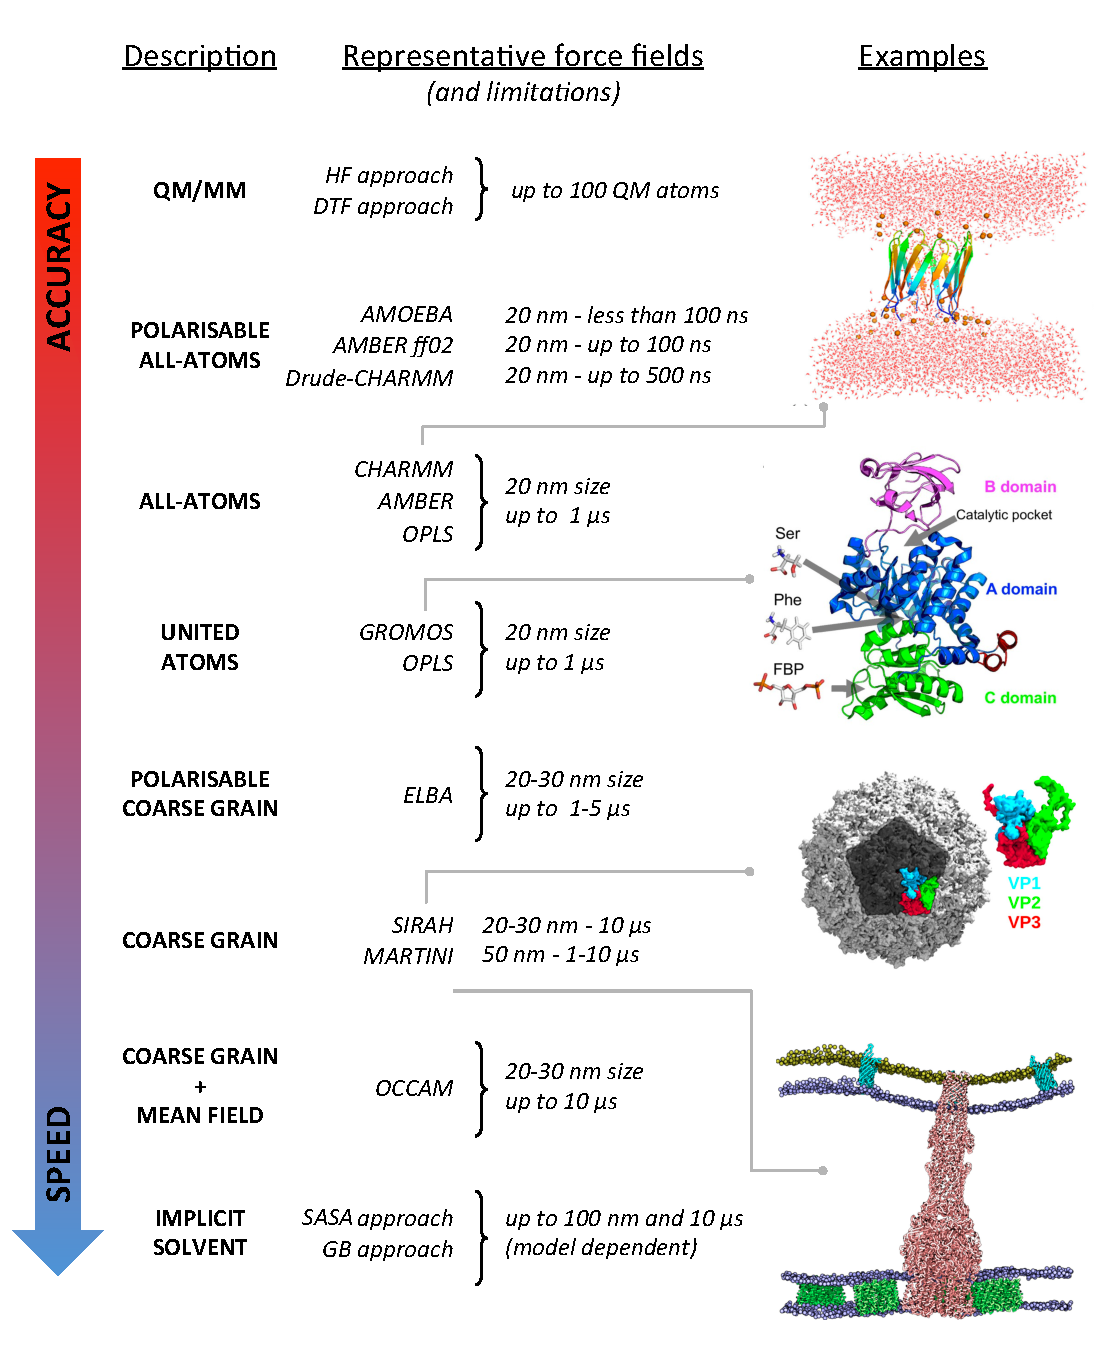
\includegraphics[scale=.65]{picture_chapter}
%
\caption{List of most popular simulation force field for biomolecules, ordered from detailed to coarse (reference to the relative papers in Section \ref{sec:ff_ex}). On the left, snapshot of notable systems simulated with the force fields CHARMM (adapted with permission from \cite{Lipkin2017}. Copyright (2017) American Chemical Society); GROMOS (adapted with permission from \cite{Macpherson2019}); SIRAH (adapted with permission from \cite{Machado2017}. Copyright (2017) American Chemical Society) and MARTINI (adapted with permission from \cite{Samsudin2017}). Copyright (2017) Elsevier).}
\label{fig:ff}
\end{figure}


Many force fields for classical MD simulations adopt a functional form equal or similar to the one described above. Their difference lies in the number of degrees of freedom modelled, in a hierarchy of descriptions proceeding from detailed to coarse  (Figure \ref{fig:ff}). Three possible classes of descriptions are:
\begin{itemize}
\item all-atoms force fields, where all the atoms are presented in the description, and represented as spheres of variable size according to their van der Waals radius (e.g. proportional to $\sigma$ in a Lennard-Jones model). Examples of all-atoms force fields are AMBER \cite{Maier2015,Dickson2014,Wang2004_amber}, CHARMM \cite{MacKerell1998,Klauda2010,Huang2013} and OPLS all-atom \cite{Jorgensen1988}.
\item united atoms force fields, similar to the previous ones but where non-polar hydrogens are incorporated in the heavy atom they are bonded to. The ``united atom" is given a new $\sigma$ parameter and increased mass according to how many hydrogen it includes. The GROMOS force field \cite{Oostenbrink2004,Schmid2011} follows this philosophy. The OPLS force field has also a united atom version \cite{Jorgensen1996}.
\item coarse grain force fields, which group together in one unique bead few atoms, to reduce the number of variables to compute. The clustered atoms are such that their mutual distances are expected to vary little with respect to the ample movements of components of the system far away from each other (which will be grouped in different beads). The MARTINI \cite{Marrink2007,Monticelli2008,DeJong2013} and SIRAH \cite{Machado2018,Barrera2019} force fields belong to this category.
\end{itemize}
%
We now give a more detailed insight in the characteristics and parametrisation strategies an atomistic and a coarse grain force field among the ones mentioned.



\subsubsection{The GROMOS force field}
All-atoms and united atoms force field are parametrised against experimental values.
%
While for the all-atom force fields AMBER and CHARMM the parametrisation is based on ab initio quantum mechanics calculations, refined against experimental data if needed \cite{Maier2015,Dickson2014,Wang2004_amber,MacKerell1998,Klauda2010}, the united atom GROMOS force field relies on the reproduction of free enthalpies of solvation and heat of vaporization of small molecules at physiological temperatures and pressures \cite{Oostenbrink2005,Schmid2011,Reif2013}.
%
This procedure sets not only the constant of the bonded interactions, but also the partial charges of the atoms inside a molecule: as no electrons are included for the sake of efficiency, their redistribution across atoms which are bonded is modelled through fractional charges assigned to each atom (while the total charge of a molecule must sum to an integer).
%
Moreover, it is assumed that the parametrisation performed for small moieties can be transferred to a larger compound including these moieties. This limits the number of chemical groups to be described in order to simulate biomolecules.

In every MD simulation, the description of water is crucial. Out of the many water model proposed, the GROMOS parametrisation has been performed with a flexible simple point charge (SPC \cite{Berendsen1981}) model. This description represents water as a three atoms molecule, with a negative charge on the oxygen and a positive complementary one on the two hydrogen atoms, and allowing flexible hydrogen-oxygen bonds. This model reproduces correctly the density and dielectric permittivity of water.

The improvement of computational techniques and reparametrisation strategies prompts the periodical release of newer versions of force fields. Accordingly, the latest version of the GROMOS force field, version 54a8 \cite{Schmid2011}, has been released in 2011.

\subsubsection{The MARTINI force field}

The MARTINI force field is a popular coarse grain description of biological molecules \cite{Marrink2007,Monticelli2008,DeJong2013}: developed originally with a focus on lipids, it has been then extended to include proteins, small ligands and DNA/RNA molecules.

MARTINI opts for a four-to-one approach, i.e.\ four heavy atoms are grouped in one bead. The number of bead types has been kept to the minimum necessary to represent biological molecules. They are organised systematically in polar, non-polar, apolar, or charged, and each type has a number of subtypes with increasing polarity to differentiate the chemical nature of the underlying atomistic structures.
%
This systematic approach can be easily transferred to new compounds, without the need of introducing new bead types.
%
The only exception is represented by rings molecules, where a two-to-one approach is needed to maintain the circular topology.

Two approaches are possible develop a coarse grain description: parameters can be fit directly to global quantities derived from experiments, in a top-down approach as the one followed in GROMOS; or fitting the coarse-grain simulations results to the ones from atomistic simulations, in a bottom-up approach.
%
The MARTINI force field chooses a top-down approach to parametrise non-bonded interactions, tuning them against experimental partitioning free energies between polar and apolar phases, while bonded interactions are derived from reference all-atom information, in a bottom-up approach.

The four-to-one mapping implies that the amino acid backbone is represented by one bead only, preventing the description of directional bonds which are key to reproduce the secondary structure. The bonded parameters partially account for this, favouring for each residue type the backbone conformation in which it is most likely found (as computed from the Protein Data Bank - PDB \cite{PDB}). When this is not sufficient, the protein can be constrained around a given structure through an elastic network model approach (ElNeDyn \cite{Periole2009}). However, both the backbone parametrisation and the use of ElNeDyn imply that conformational changes in the structure are penalised and therefore not well sampled in MARTINI simulations.

The MARTINI force field provides two water model. The standard one groups four water molecules in one bead only, loosing the polarisability typical of water molecules, the effect of which is partially restored with the use of a high dielectric constant. The polarisable water model \cite{Yesylevskyy2010} maps instead four water molecule to a single ``inflated" water, i.e.\ a three-beads molecule with the same shape of a single molecule, but expanded, and a charge splitting which can account for the water dipole.

\runinhead{Backmapping techniques} Coarse-grain descriptions are very effective in reproducing long time scales; however, to retrieve finer details after such extensive exploration, backmapping techniques have been designed to obtain atomistic configurations from the coarse-grain ones \cite{Wassenaar2015}. The easy transfer between the two resolution, gave rise to many multiscale studies applied to biomolecular systems \cite{Lee2012}.


\subsection{Beyond a classical atomistic framework} 

Without entering into the details, we want to bring to the reader attention two possible refinements of the aforementioned models, and two computational strategies which on the contrary speed up the calculations at the expenses of the loss of some details.

Regarding the accuracy of simulations, it must be noticed that none of the force field mentioned above takes into account polarisability, i.e. the displacement of electrons with respect to the nucleus, as a consequence of the surrounding electrostatic environment, because electrons and nucleus of an atom are modelled as a unique object. Specific force fields have been modelled to include this effect, on top of atomistic descriptions, as in the AMOEBA \cite{Ren2003,Ponder2010}, Drude polarisable CHARMM \cite{Anisimov2004} or AMBERff02 \cite{Cieplak2001}, or on coarse grain descriptions, as in the ELBA force field \cite{Orsi2011}. Polarisability does improve the accuracy of simulations, but it can significantly slow down simulations.
%
Going beyond the classical approximation, for biological processes governed by quantum mechanics - such as photosynthesis, DNA mutation processes or some enzymatic activities - many semi classical hybrid techniques have been developed \cite{Ahmadi2018}. They combine computational quantum mechanical modelling methods, such as Density Functional Theory (DFT) or Hartree-Fock computations (HF) \cite{Shao2015}, with classical Molecular Dynamics to gain the accuracy of a quantum description in the region of interest and the speed up of a classical one in the surrounding areas.

Tackling instead efficiency issues, an implicit solvent model can be used to speed up simulations. The solvent is represented as a continuous medium, as opposed to explicit models which include all its particles \cite{Kleinjung2014}.
% In this situation the description of the solute is usually, but not necessarily, atomistic as the speed up gained by this solvent parametrisation allows a very detailed description for it.
%
Models of implicit solvent can be based on different assumptions: for example the solute-solvent interactions can be taken as proportional to the solvent-accessible surface area (SASA) of every particle of solute \cite{Fraternali1996,Kleinjung2003,Kleinjung2012,Fornili2012}, or instead can be derived from a solution of the Poisson-Boltzmann equation governing the charge density in a material, for example in the form of the Generalised Born equation \cite{Zhu2005} which is valid under particularly simple conditions.
%
Another speed up technique is constituted by hybrid particle-field algorithms. The idea is to treat non-bonded interactions through a mean field approach, where atoms/beads move in the field generated by the others. The field does not need to be updated at every time step, as it is a collective and thus slowly evolving variable; moreover, for each particle only the interaction with the field, and not with all the neighbour particles needs to be computed, reducing the computations effort further. This approach has been employed with a coarse grain description of polymers and biological molecules in the OCCAM software \cite{Milano2009}.

Finally, further strategies are possible to enhance the sampling performed by a simulation in the case that the one obtained by the natural evolution of the system would exceed the computational time available. As a non comprehensive list of these techniques, we mention replica-exchange algorithms \cite{Okamoto2004} which combine together multiple simulations held at different conditions, local potential-energy elevation (or metadynamics) \cite{Huber1994,Laio2002} which avoids the re-sampling of already visited conformations adding an energy penalty to them, umbrella sampling \cite{Torrie1977} which reconstructs free-energy barriers from simulations held at specific values of the coordinate along which the barrier exists, or finally simply the use of higher temperature to overcome energy barriers \cite{Kirkpatrick1983}.

\subsection{System setup}
To set up a simulation, the desired resolution, i.e. force field, must be chosen according to the system to simulate. A few examples on this will be given in Section \ref{sec:methods}; however, for any choice of parameters, some common ``ingredients" and steps are necessary to prepare the system:
\begin{itemize}
\item \textbf{structural file}: a pdb file (or any structural file format suitable with the MD engine of choice) which contains only the elements to be simulated, with a correct format of names and positions. The choice of the initial conformation is particularly important, especially for atomistic resolution, which is likely to sample conformations in the vicinity of the initial position if it possible to simulate only a short time scale.
\item \textbf{topology file}: given a structural file, every MD engine has dedicated commands to retrieve the list of parameters for bonded atoms. The presence of exotic residues or non standard network of bonds might need case-to-case manual parametrisation.
\item \textbf{simulation box}: for simulations of a protein, it is good practice to place it within a box large enough to avoid interference of the protein with its periodic images, for example allowing a minimum distance between protein and box of at least the cut-off chosen for non-bonded interactions. However, it must be considered that the protein might adopt extended conformations extend during the simulation, therefore one should find a compromise between the needed box size and the effective number of particles to calculate.
%
In the case of lipids instead, to reproduce an infinite membrane and account for lateral tension, the box can be chosen exactly as big as the membrane patch (in the directions parallel to its plane), so that periodic images merge together.
\item \textbf{solvation}: the prepared box is filled with molecules of the water model of choice, except in the spaces already occupied by the solute.
\item \textbf{ions}: ions are added in replacement of a suitable number of water molecules to neutralise the charge of the system. Additional ones can be added to reach the experimental ion concentration (though there will be a slight imbalance between the positive and negative species due to the counter ions already added).
\item \textbf{energy minimisation}: the system prepared according to the steps above might have several atom clashes. This can derive from the initial protein/membrane structure, or from imperfect packing of the solvent around the solute. To alleviate this, an energy minimisation is performed prior to the dynamical run. Usually, a protocol restraining the  the solute and letting relax solvent positions in the first instance, followed by a second run that releases the solute is used in these cases.
\item \textbf{equilibration}: even after energy minimisation, the system prepared is far away from the ideal equilibrium configuration. For this reason, several rounds of simulations with specific conditions are run before the final production. The specific protocol depends on the system and the force field, however for proteins in solution it is quite common to start with NVT ensemble runs with position restraints at increasing temperatures, followed by NPT runs at the same temperatures but without restraints, and only then from the production. For lipid system, the simulated ensemble is preferably NPT to prevent penetration of water in the bilayer by unphysical shrinking the box. After this only a temperature increase protocol is followed. In some cases, for example for the MARTINI force field with standard water, it is not possible to simulate low temperatures, thus the equilibration consists in a short production employing different thermostat and barostat with respect to the production. Some of these protocols are more suitable for approaching efficiently the correct temperature or pressure value from a configuration far from equilibrium, while others for maintaining the correct ensemble properties. Generally, every force field is provided with validated equilibration procedures.
\end{itemize}


\section{Methods: relevant examples} \label{sec:methods}
One of the challenges of MD simulations consists in choosing the most suitable granularity of the description, together with the choice of the system to simulate. We list here a few examples which might convey better the idea of suitable setup  for systems of current interest.

\runinhead{Simulations of protein and their interactions}
Simulations of protein have been crucial to understand small molecular details of their structure and functioning, which influence their macroscopic behaviour.

A challenging subject in the field of enzymatic regulation is constituted by allosteric regulation, as the pathways involved are of difficult exploration. Molecular dynamics simulations can shed light on the residues responsible for transferring the information \cite{Pandini2012}.
%
For example, atomistic simulations of pre-assembled pyruvate kinase M2 (PKM2) tetramers elucidated the mechanism of allosteric activation by fructose 1,6-bisphosphate (FBP) \cite{Macpherson2019}. In this work, the correlated motions extracted from simulations of the apo and FBP bound tetramer were processed within an information-theoretical framework, allowing for the extraction of specific residue hubs.  These were experimentally demonstrated to be responsible of the communication between ortosteric and allosteric pockets.

Another particularly interesting concept explored by MD is the one of \emph{ensemble}: proteins adopt a variety of shapes in solution, which can differ significantly from the crystal-structures available. This flexibility is proven by techniques as small angle X-ray scattering (SAXS) or nuclear magnetic resonance (NMR), which results cannot been explained by a single-conformation scenario. As such, simulations can provide ``snapshots" of all these conformations and their mutual interchange.
%
Some of these changes are crucial for the protein function, as in the case of prions, proteins which become pathogenic under conversion from an $\alpha$-helix rich form to a $\beta$-sheet isoform which is prone to aggregation. 
Atomistic MD simulations of the prion protein showed the (reversible) unfolding of the protein between the two structural states \cite{Chakroun2013}, starting from the helical crystal structure available. Moreover, they identified in the C-terminus region the trigger of the conformational change, corresponding to a region which is enriched in pathogenic mutations. The results were then used to investigate the aggregation process after the conversion, again identifying critical residues promoting it \cite{Collu2018}. 
Interestingly, the water distribution density around the prion molecule was demonstrated to have a role in identifying possible spots prone to aggregation \cite{DeSimone2005,DeSimone2006}. Such examples show that one should consider the solvent, or the forces induced by the protein surrounding media, as an important determinant in the conformational equilibria and recognition processes.
%
Assembly simulations applied to amyloid forming peptides has provided recently a map of all the relevant states of the assembly process \cite{Sengupta2019}, suggesting that the constant improvement of computational power will make this possible also for more complex systems like the prion in a near future.


\runinhead{Simulations of model membranes} 
Membrane simulations had a key role in elucidating the mechanical and dynamical characteristics of these important organelles clarifying for example how the lipids composing the membrane influence its fluidity \cite{Risselada2008,Song2019}, or elucidating the interactions between lipids and surface proteins, transmembrane ones or membrane active peptides, such as antimicrobial ones \cite{Leontiadou2006,Ulmschneider2017,Sun2015}.

The last point in particular raised the interest in simulating bacterial membranes. As these objects are very complex, simplified models can be used to approach the problem.
%
Very often, these models use only one or two lipid species to represent membranes, e.g. bacterial ones have contains neutral phospholipids with a percentage of negatively charged ones \cite{Lipkin2017,Wang2012,Zhao2018,Chen2019} as key characteristic distinguishing them from mammal membranes, which possess only zwitterionic phospholipids, with the occasional inclusion of cholesterol, deemed important in achieving the flexibility typical of mammal membranes \cite{Lipkin2017,Wang2012,Zhao2018,Chen2019,Risselada2008}.
%
Because of their simplicity, these systems are extensively used also in experiments \cite{Castelletto2016,Tang2009,Glukhov2005}, making a direct comparison with simulations possible. Nevertheless, attempts to model more accurately cell membranes have been pursued.

The atomistic level is suitable to reproduce single components of the membrane, e.g. the isolated inner membrane of Gram-negative bacteria \cite{Piggot2011}, even if atomistic computations started in recent years to be affordable also for larger systems.
%
For example, atomistic simulation of the outer membrane of Gram negative bacteria combined with the peptoglycan layer (which is positioned between the two membranes) elucidated how the distance is variable, thanks to the presence of Braun's lipoproteins which act as a bridge between the two, and can bring them closer by bending and tilting \cite{Samsudin2017}.
%
Moreover, the permeability of membranes to ions and small compounds needs to be assessed at the atomistic level to get sufficient accuracy, and because of the intensive task, often enhanced MD techniques such as umbrella sampling are employed \cite{Carpenter2016}.

Coarse grain descriptions are instead the most suitable to represent the full bacterial envelope, especially in the case of Gram-negative bacteria, as the inclusion of all its elements results in large systems.

Accordingly, MARTINI simulations have been able to reproduce the behaviour of several transmembrane proteins which spanned both the inner and outer membrane \cite{Hsu2017} and to model all the different components of the Gram-negative cell envelope \cite{Khalid2019}.
%
Similarly, the ability of coarse grain simulations to investigate very large systems makes them suitable to assess elastic properties of membranes, as they can access low frequency undulations with little influence from finite size effects \cite{Fowler2016}.


\section{Notes: validation and challenges of MD simulations}

Validation of MD simulations is performed by comparison with experiments: the same properties obtained experimentally are computed from the MD trajectory as well, and the two compared. If these are correctly reproduced, it is usually assumed that the simulation is sampling the correct ensemble of states and then one can identify in the simulation the determinants responsible for the experimental outcome of interest, which are not accessible by the experiment itself.

The comparison however is not always easy: often the experimentally measured quantity is an average in time and/or space (for example Circular Dichroism spectra or SAXS profiles of a peptide in solution) and many different combinations of computationally derived structure ensembles can produce compatible results. It is still challenging to compare experimentally derived ensembles and the ones derived by molecular simulations. Indeed the extracted average properties may be different, so it is important to understand which are the relevant properties playing a role in the measured ensemble before attempting comparisons.

Thus, in the validation of MD outcomes, it is important to have a critical attitude and to interpret the result within the validity of the approximation \cite{VanGunsteren2008}. Some apparently negative results may suggest or stimulate new experimental settings to validate the hypotheses one was set to test \cite{Goncalves2013,Meissner2014}.
%
Indeed, agreement may arise from either a simulation that reflects correctly the experimental system; but also when the property examined is insensitive to the details of the simulated trajectory, or it can be a result of compensation of errors, which is more likely to  occur for systems with a high number of degrees of freedom.
%
Similarly, disagreement may hint at an error in the simulation (either in the model, the implementation, or simply the estimated simulation's convergence) or an error in the interpretation and/or conditions of experimental set-up (either in the result itself o its interpretation), so that both must be carefully checked to improve a convergence in the agreement.

Finally, simulations still suffer from the limited computational time available: most of the times, the real experimental system is simply too large to be reproduced and the time scale of the process too long. Simulations are thus confined to explore a restricted space, implying that the initial conditions must be chosen carefully to optimise the search and avoid any bias which might persist for the whole length of the simulation. The use of enhanced MD techniques can increase the chances of sampling relevant states, however it introduces a bias which must be removed or properly accounted for in the interpretation of the results \cite{Bernardi2015,Best2005,Barducci2010,Barducci2011,Mills2008}.
% Bernardi2015 general; Best2005 REX; Barducci2010,Barducci2011 metadynamics; Mills2008 umbrella sampling
Finally, one should keep in mind that the force fields used are far from optimal. Partly because they rely on approximate functional forms, and partly because it is difficult to find experimental observables measured with the desired resolution able to discriminate between sets of parameters.

It remains important to note the contribution that Molecular Dynamics simulations have played in disclosing important details behind biophysical processes and in unravelling molecular details not accessible to experiments.
% cite rev

%\printbibliography
%\bibliographystyle{naturemag}
\bibliographystyle{my_bib}
\bibliography{thesis_ref2.bib}
%\input{references}

\end{document}
